% \begin{figure}
%   \centering
%   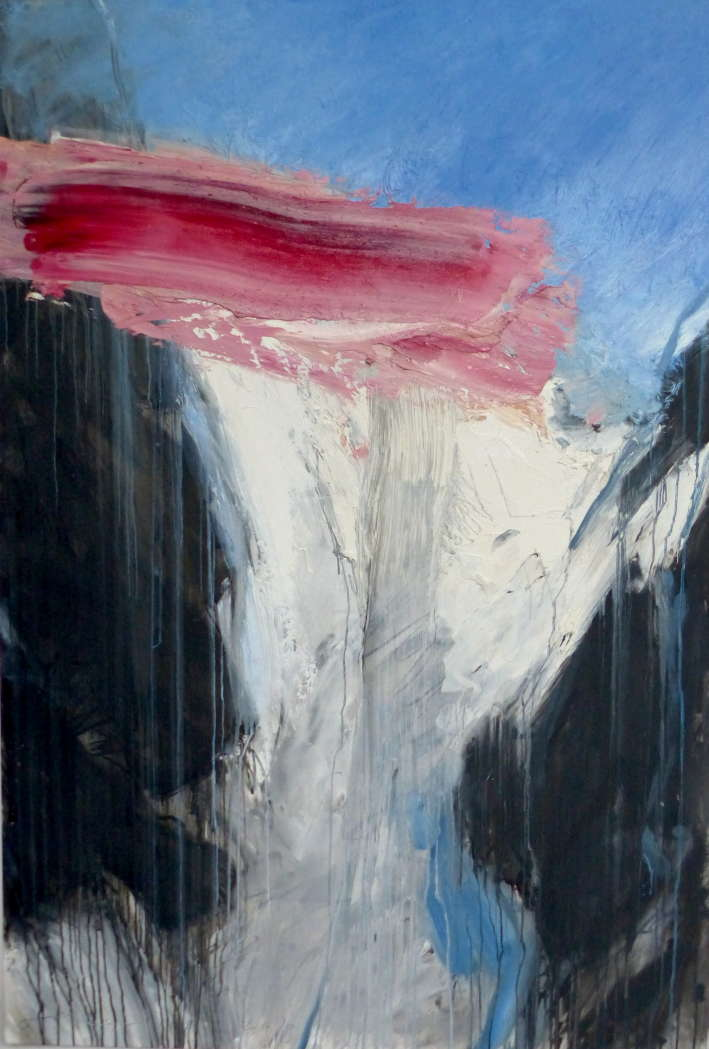
\includegraphics{./figures/Le_couloir_Rochette.jpg}
%   \caption{\emph{Le couloir,} Jean-Marc \bsc{Rochette,} 2010.}
%   \label{fig:couloir_rochette}
% \end{figure}

Notre mémoire de thèse est organisé en trois parties, regroupant neufs
chapitres. La première partie vise à présenter le cadre de ce travail,
qu'il soit applicatif, organisationnel ou scientifique.  Dans le
premier chapitre de cette partie nous présentons le contexte
applicatif et organisationnel de la thèse. Nous aborderons ensuite,
dans le second chapitre, le contexte scientifique de la thèse et nous
définirons la problématique du sujet. Enfin, dans le troisième
chapitre nous dresserons un état de l'art sur les questions
principales de ce travail.
%
La seconde partie est destinée à présenter notre méthode de
transformation des positions exprimées dans un référentiel indirect en
des zones de localisation. Elle est constituée de cinq chapitres. Le
premier chapitre de cette partie présente l’organisation générale de
notre méthode. Les chapitres suivants approfondissent des points
spécifiques de cette méthode. Dans le \autoref{chap:05} nous
détaillerons le fonctionnement de la première phase de la méthode,
\emph{la décomposition.} Le \auotref{chap:06} sera quant à lui
consacré a la définition d'un modèle permettant la représentation
d'objets géographiques imprécis, tels que ceux produits par notre
méthode. Dans le \autoref{chap:07} nous présenterons la seconde phase
de notre méthode, \emph{la spatialisation.} Le dernier chapitre de
cette seconde partie sera consacré à la présentation de la dernière
phase de notre méthode, la \emph{fusion.}
%
La troisième partie de ce manuscrit présente l’application de la
méthode définie a plusieurs alertes réelles. Cette partie ne contient
qu'un seul chapitre, le neuvième, où trois alertes réelles sont
présentées.

